\section{Numerical experiments}
\label{sec:numerics}

Two benchmarks examine geometric efficiency and the consequences of deployment shift. Their nominal plants are retained from the submitted examples. The disturbance generators are specified anew to satisfy the revised statistical assumptions. The code supplies independent data streams and all geometric checks; counterexamples and rejected designs are retained as diagnostics.

\subsection{Common protocol and baseline calibration}
\label{subsec:numeric-protocol}

The stage cost is $\ell(x,u)=x^\T Qx+Ru^2$. Set $K_f=K$ and use $V_f(z)=z^\T Pz$, where $P$ solves
\begin{equation}
 A_K^\T PA_K-P=-(Q+K^\T RK).
 \label{eq:numeric-terminal-cost}
\end{equation}
Independent streams provide 1,800 design trajectories and 50,000 calibration trajectories per context. Separate tests use 80,000 trajectories per context. Each main comparison uses 120 missions of $T=22$ steps, with paired initial states and primitive random streams. Initial modes have the stationary law of their exogenous chain. The common trajectory-risk target is $\beta=0.004$ and the confidence allowance is $\delta=0.001$ per method and experiment. The mission budget is $B_0=\varepsilon=0.1$; the continuation-reserve constraint is enforced for every certified controller. A simultaneous confidence claim across all comparisons would require further allocation.

Preliminary half-widths are design-sample root-mean-square values, bounded below by $10^{-8}$. The \emph{compatibility-first atlas} applies \eqref{eq:box-closure} before calibrating \eqref{eq:compatible-score}. For $G=|\calG|$ contexts, the prescribed discard count and reference charge are
\begin{equation}
 s=\max\{j:B_{N_g}(j;\beta)\le\delta/G\},\qquad
 \bar r^0=U(N_g,s,\delta/G).
 \label{eq:numeric-rank}
\end{equation}
The \emph{calibrate-then-close ablation} first calibrates the raw RMS score and then enlarges its boxes by closure. The \emph{no-edge diagnostic} retains those raw boxes. The \emph{global comparator} uses the common shape given by the componentwise maximum of the context RMS shapes, then applies compatibility-first calibration under each conditional law and takes the largest threshold.

The \emph{Bonferroni box} calibrates $d=nH$ absolute-coordinate margins at risk $\beta/d$ and confidence $\delta/(Gd)$, and sums their certified risks. The \emph{scenario box} contains the first $N_s$ complete trajectories using their coordinatewise absolute maxima. This is the unique minimizer of the sum of $d$ nonnegative half-widths subject to sample containment. Its dimension-dependent scenario bound is $B_{N_s}(d-1;\beta)$ \citep{CampiGaratti2008}; choose the smallest $N_s$ making this at most $\delta/G$. Both boxes undergo edge closure and terminal validation. These parameterizations represent specific baselines; alternative scenario-PRS constructions can have different effective dimensions.

Cost is the mean realized sum $\sum_{k<T}\ell(x_k,u_k)$. State tightening averages $s_{t,j}^c/x_{\max,j}$ over $t=1,\ldots,H$ and coordinates; input tightening averages $|K|s_t^c/u_{\max}$ over $t=0,\ldots,H-1$. Mission averages use the selected charts. Horizon escape is evaluated on ancillary continuations coupled to the actual first disturbance. The controlled kernel in Benchmark B is evaluated on each continuation's own state/input path. Physical violations and first-error escapes are logged separately.

Condensed convex QPs use SLSQP with analytic derivatives and tolerance $10^{-10}$. Acceptance requires successful termination and a primal residual below $2\cdot10^{-7}$; a separate LP feasibility check precedes a geometric rejection. The code also checks every stored edge and all terminal conditions in \eqref{eq:numerical-terminal-checks}.

\subsection{Benchmark A: a sufficient Markov context}
\label{subsec:numeric-A}

The double integrator is
\begin{equation}
 A=\begin{bmatrix}1&1\\0&1\end{bmatrix},\quad
 B=\begin{bmatrix}1/2\\1\end{bmatrix},\quad
 K=\begin{bmatrix}-0.717&-1.061\end{bmatrix},\qquad H=8,
 \label{eq:benchA-system}
\end{equation}
with $Q=\diag(1,0.18)$, $R=0.025$, $x_{\max}=(8,4)^\T$, and $u_{\max}=1.55$. Initial states are uniform on $[-6,6]\times[-0.6,0.6]$. The observed exogenous regime has transition matrix
\begin{equation}
 P_{\rm G}=\begin{bmatrix}
 0.970&0.025&0.005\\0.250&0.730&0.020\\0.150&0.100&0.750
 \end{bmatrix}.
 \label{eq:numeric-A-transition}
\end{equation}
Use \eqref{eq:markov-noise-model} with independent $\eta_k\sim\mathcal N(0,I_2)$ and
\begin{align}
 L_0&=0.25\begin{bmatrix}0.020&0\\0&0.030\end{bmatrix},&\mu_0&=(0,0)^\T,\nonumber\\
 L_1&=0.25\begin{bmatrix}0.055&0.020\\0.012&0.095\end{bmatrix},&\mu_1&=0.25(0.015,-0.010)^\T,\label{eq:benchA-noise}\\
 L_2&=0.25\begin{bmatrix}0.130&0.065\\-0.015&0.165\end{bmatrix},&\mu_2&=0.25(-0.020,0.015)^\T.\nonumber
\end{align}
The context evolves throughout every prediction horizon. Its current value determines the future residual law independently of the selected tail, establishing the matched-law assumption exactly.

\begin{table}[tb]
\ifmarkchanges\color{blue}\else\color{black}\fi\centering\small
\setlength{\tabcolsep}{3pt}
\caption{Benchmark A: calibration and mission accounting, with $B_0=0.1$. Confidence is per context for scalar/scenario calibration and per absolute-coordinate margin for Bonferroni. Scalar shapes additionally use 1,800 independent design trajectories per context. The displayed spending and final balances hold in every main-run mission.}
\label{tab:calibration-budget}
% Generated from experiments/results by experiments/make_paper_assets.py.
\begin{tabular}{lrrrrrr}
\toprule
Construction & $N$ used & Confidence & $s$ & Chart charge & $\sum_k p_k$ & $B_T$ \\
\midrule
Collective score & 50,000 & $\delta/3$ & 153 & 0.003993875 & 0.087865 & 0.012135 \\
Bonferroni box & 50,000 & $\delta/48$ & 0 & 0.003448894 & 0.075876 & 0.024124 \\
Scenario box & 8,295 & $\delta/3$ & 0 & 0.003999847 & 0.087997 & 0.012003 \\
\bottomrule
\end{tabular}

\end{table}

\Cref{tab:calibration-budget} specifies the common $(\beta,\delta)$ comparison. Bonferroni uses all 50,000 samples with zero discards, whereas the scenario box uses 8,295 samples and leaves the remainder unused. Thus the two coordinatewise maxima, and their resulting tightenings, differ. All three verified constructions have the same class of containment-based feasibility and mission-risk guarantee. The smallest calibration counts admitting these respective finite certificates are 1,998 for the scalar family, 8,295 for the dimension-16 scenario box, and 43,111 for the equal-allocation Bonferroni box. The scalar count excludes its independent design split; statistical admissibility still requires subsequent geometric checks.

\begin{table}[tb]
\ifmarkchanges\color{blue}\else\color{black}\fi\centering\small
\setlength{\tabcolsep}{3pt}
\caption{Benchmark A: 120 missions per row. Horizon is the escape percentage over 2,640 decisions; Test is the largest of three independent context-conditional escape percentages. Tightening and Feas. entries are percentages. Feas. is the stationary-context-weighted fraction of nominally feasible grid states. Every row except the no-edge diagnostic verifies all nine transitions and terminal conditions.}
\label{tab:benchA-results}
% Generated from experiments/results by experiments/make_paper_assets.py.
\begin{tabular}{lrrrrrr}
\toprule
Method & Cost & Horizon & Test & $X$ tight. & $U$ tight. & Feas. \\
\midrule
Compatibility-first & 25.879 & 0.2652 & 0.2988 & 5.10 & 25.82 & 88.01 \\
Calibrate then close & 25.912 & 0.0000 & 0.0000 & 9.33 & 47.42 & 81.02 \\
Global, compatible & 25.929 & 0.0000 & 0.3425 & 5.68 & 29.44 & 86.81 \\
Bonferroni atlas & 25.887 & 0.0000 & 0.0037 & 7.01 & 35.50 & 86.83 \\
Scenario-box atlas & 25.884 & 0.0000 & 0.0325 & 6.46 & 32.60 & 87.38 \\
No-edge diagnostic & 25.890 & 0.1894 & 0.3387 & 2.16 & 11.30 & -- \\
\bottomrule
\end{tabular}

\end{table}

Every row in \Cref{tab:benchA-results} completes all missions without physical violations or reset failures. Compatibility-first calibration has seven horizon escapes and seven first-error escapes. Its independent conditional escape rates are $0.29875\%$, $0.29625\%$, and $0.27750\%$. The no-edge diagnostic fails 89 scalar inclusion tests and verifies none of its nine candidate edges; sampled feasibility supplies no atlas-level recursive-feasibility certificate for that row. All budgets remain nonnegative. The calibrate-then-close and global constructions have the same charge and mission spending as the scalar row of \Cref{tab:calibration-budget}. The no-edge row debits that reference charge diagnostically, without claiming the certified continuation property.

Compatibility-first calibration reduces both tightening measures by approximately $45\%$ relative to calibration before closure. Its cost advantage over the scenario box is only about $0.02\%$. The main gain is geometric: LP tests on a $61\times41$ grid in $[-8,8]\times[-4,4]$ give the feasible-domain comparison in the table. These percentages describe the sampled nominal domain, rather than a probability of closed-loop success. Median QP times in these runs are approximately 1 ms, offering no evidence of a computational-speed advantage.

\begin{figure}[tb]
\ifmarkchanges\color{blue}\else\color{black}\fi\centering
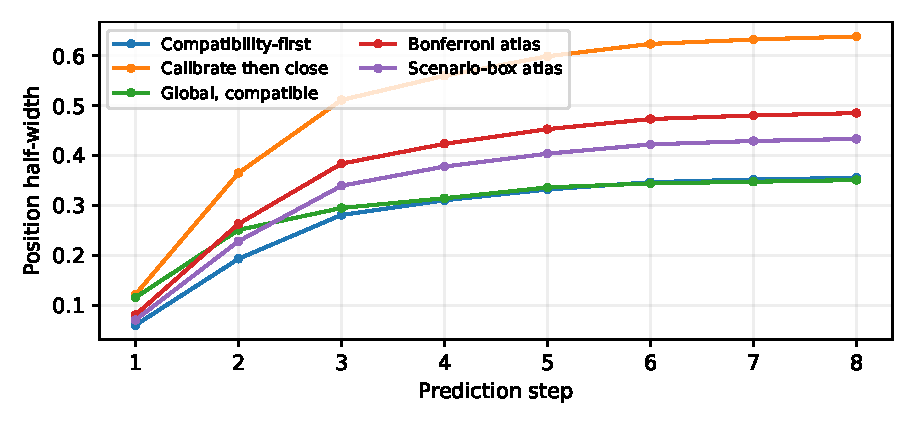
\includegraphics[width=.91\linewidth]{figures/benchmark_A_tightening.pdf}
\caption{Benchmark A: position half-widths, averaged equally over contexts. Calibrating the compatible templates substantially reduces later-section enlargement.}
\label{fig:benchA-tightening}
\alttext{Five curves compare position half-widths over eight prediction steps. Compatibility-first calibration has smaller later-section margins than the global and coordinatewise comparators. Calibration before closure gives the largest later-section margins.}
\end{figure}

\paragraph{Data fairness and replication.}
Using the same total pool of 8,295 trajectories per context as the scenario box, the collective method reserves 1,800 for design and 6,495 for calibration. Its state/input tightenings are $5.41\%/27.37\%$, compared with $6.46\%/32.60\%$ for the scenario box; costs are $25.880$ and $25.884$. Its charge is $0.003982643$, giving spending $0.087618$ and final balance $0.012382$. This comparison accounts for the design-data requirement explicitly.

Three further independent design/calibration replications retain the geometric ranking against the implemented verified baselines. Across the four full-sample runs, collective state tightening ranges from $5.05\%$ to $5.14\%$ and input tightening from $25.54\%$ to $26.02\%$. All 480 missions complete without physical violations or reset failures. One replication has an observed horizon-escape frequency of $0.5682\%$, above the $0.4\%$ target; all independent conditional tests remain below it. Such finite empirical frequencies fluctuate, and overlapping horizon indicators provide no independent-binomial mission sample. All replication logs are included.

\paragraph{Why conditional calibration matters.}
A separate pooled-score diagnostic uses stationary initial-mode weights $(0.88394,0.09109,0.02497)$. Its mixture-weighted test escape is $0.3387\%$, while escape conditional on the rare third mode is $8.4013\%$. This is a mixture-law calibration diagnostic, with no chart-switching claim. The global comparator in \Cref{tab:benchA-results} instead certifies every conditional law, avoiding that mismatch.

\subsection{Budget continuation and nominal recovery}
\label{subsec:numeric-operations}

For a tighter mission budget, use two risk levels in each context:
\begin{equation}
 (\beta_{g,h},\beta_{g,l})=
 (0.0040,0.0012),\ (0.0037,0.0015),\ (0.0031,0.0018)
 \quad(g=0,1,2).
 \label{eq:numeric-context-risks}
\end{equation}
The six preliminary templates multiply the RMS widths by their design-sample $(1-\beta_{g,\cdot})$ score quantiles. Apply closure, allocate confidence $\delta/6$, and calibrate one common scale. All 36 edges and terminal conditions pass. Forty missions with $B_0=0.065$ and penalty $10^{-3}\sum_{t,j}s_{t,j}^c$ yield 12 different risk-level schedules. Spending lies between $0.062348$ and $0.064881$, with smallest final balance $0.000119$. All missions complete without escapes or physical violations. This test uses the complete context graph and illustrates context-dependent charging with a continuation reserve.

For comparison, a current-affordability-only run using the single-rate atlas and $B_0=0.02$ exhausts its budget after five contained steps, spending $0.019969$. The reserve admission test rejects that same 22-step specification before applying an input because it requires $0.087865$. Budget exhaustion thus needs no realized failure.

A separate recovery stress test starts at $(1,0.1)^\T$ and adds $(6.5,3)^\T$ to the disturbance at $k=3$. It is excluded from stochastic coverage estimates. At $k=4$, the state is approximately $(6.4969,2.9933)^\T$, inside the state box but outside the reset-feasible domain. Conditional initialization supplies 14 feasible recovery QPs through step 17. Projection preserves the input bound, while four subsequent states violate the state constraints. This separates current state admissibility from recoverable nominal feasibility. Statistical charging ends at recovery entry, after spending $0.015975$.

\subsection{Benchmark B: state/input-dependent deployment shift}
\label{subsec:numeric-B}

The mass-spring example uses
\begin{equation}
 A=\begin{bmatrix}1&0.35\\-0.2275&0.937\end{bmatrix},\quad
 B=\begin{bmatrix}0.06125\\0.35\end{bmatrix},\quad
 K=\begin{bmatrix}-1.371&-1.713\end{bmatrix},\quad H=10,
 \label{eq:benchB-system}
\end{equation}
with $Q=\diag(1,0.25)$, $R=0.08$, $x_{\max}=(4.5,3)^\T$, and $u_{\max}=4$. Initial states are uniform on $[-3.2,3.2]\times[-0.5,0.5]$. The observed regime and innovation matrices are
\begin{equation}
 P_{\rm G}=\begin{bmatrix}0.96&0.04\\0.18&0.82\end{bmatrix},\quad
 L_0=0.4\begin{bmatrix}0.012&0\\0.002&0.018\end{bmatrix},\quad
 L_1=0.4\begin{bmatrix}0.030&0.010\\-0.004&0.042\end{bmatrix}.
 \label{eq:numeric-B-noise}
\end{equation}
Each reference step independently chooses $L_g\eta$ or $3L_g\eta$, with $\eta\sim\mathcal N(0,I_2)$ and heavy-component probability $\alpha_0=0.05$. Deployment uses
\begin{align}
 \alpha_\star(x,u)&=\alpha_0[1+(\Gamma^{1/H}-1)h(x,u)],\nonumber\\
 h(x,u)&=\tanh\bigl((x_1/2)^2+(x_2/1.5)^2+(u/2)^2\bigr).
 \label{eq:numeric-B-mixture}
\end{align}
The tested range $1\le\Gamma\le3^{10}$ gives valid probabilities. The heavy-weight ratio is at most $\Gamma^{1/H}$ and the light-weight ratio at most one. \Cref{prop:mixture-domination} therefore proves the trajectory factor $\Gamma$ uniformly over every selected tail, including its state/input dependence.

At $\Gamma=3$, the corrected atlas calibrates at $\beta/3$ with confidence $\delta/2$ per context. Its deployment charge is $0.003997602$, giving $\sum_kp_k=0.087947$ and $B_T=0.012053$ in every mission. It completes all 120 missions without physical violations, reset failures, or budget exhaustion. State/input tightenings are $11.91\%/28.17\%$, and mean cost is $10.969$. The uninflated diagnostic has $9.61\%/22.75\%$ tightening and essentially the same cost. Its unadjusted spending is $0.087638$; the justified shift-adjusted spending would be $0.262914$, failing the $0.1$ admission requirement. Consequently that row is diagnostic operation only.

The sweep in \Cref{tab:shift-sweep} uses the same reference samples and paired test streams. Independent tests execute nominal $K$-feedback tails from $[-2.4,2.4]\times[-0.35,0.35]$, using 80,000 trajectories per context. Their finite empirical rates concern those specified tails; uniform validity comes from the density-ratio proof. Additional accepted settings use 40 missions per variant. Every corrected mission completes without physical violations or reset failures.

\begin{table}[tb]
\ifmarkchanges\color{blue}\else\color{black}\fi\centering\small
\setlength{\tabcolsep}{3pt}
\caption{Benchmark B: shift-severity sweep. $N_{\min}$ is the minimum scalar calibration count per context; 50,000 are available. Tightening is for the corrected atlas, and test columns give the largest conditional escape percentages. The last column is corrected mission spending with $B_0=0.1$; its difference from $0.1$ gives $B_T$. Rejected designs have no corrected performance entry.}
\label{tab:shift-sweep}
% Generated from experiments/results by experiments/make_paper_assets.py.
\begin{tabular}{rrrrrrr}
\toprule
$\Gamma$ & $100\alpha_{\max}$ & $N_{\min}$ & $U$ tight. & Uninflated & Corrected & $\sum_k p_k$ \\
\midrule
1 & 5.00 & 1,897 & 22.82 & 0.3162 & 0.3162 & 0.087638 \\
3 & 5.58 & 5,697 & 28.17 & 0.3312 & 0.0975 & 0.087947 \\
10 & 6.29 & 18,999 & 37.10 & 0.3625 & 0.0087 & 0.083830 \\
25 & 6.90 & 47,502 & 48.23 & 0.3887 & 0.0013 & 0.083604 \\
100 & 7.92 & 190,019 & -- & 0.4338 & -- & Reject \\
59,049 & 15.00 & 112,206,419 & -- & 0.7388 & -- & Reject \\
\bottomrule
\end{tabular}

\end{table}

The corrected designs at $\Gamma=100$ and $\Gamma=59{,}049$ are rejected for insufficient calibration data. At the largest shift, the uninflated context-conditional escape rates are $0.59625\%$ and $0.73875\%$. Simultaneous two-sided $95\%$ binomial intervals have lower endpoints $0.5369\%$ and $0.6725\%$, both above the target. At that severity, the stated uniform correction requires over 112 million calibration trajectories per context. The example thus exhibits undercoverage when shift is ignored and the sample cost of a conservative trajectory-law bound. All accepted designs and rejections are reported, rather than selecting only favorable cases.

\begin{figure}[tb]
\ifmarkchanges\color{blue}\else\color{black}\fi\centering
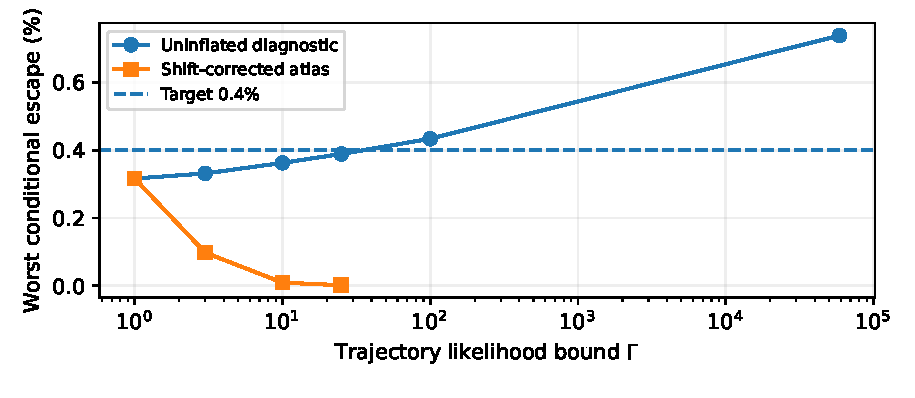
\includegraphics[width=.91\linewidth]{figures/benchmark_B_shift.pdf}
\caption{Benchmark B: worst conditional test escape versus trajectory shift bound. The last two corrected designs are unavailable with the prescribed calibration sample.}
\label{fig:benchB-shift}
\alttext{On a logarithmic shift-factor axis, uninflated test escape rises above the 0.4 percent target at large shifts. Corrected test escape stays below target at accepted settings. Corrected points at the final two settings are absent because calibration is rejected.}
\end{figure}

The numerical advantage in Benchmark A concerns the specified tube geometry and persists at matched total data. Cost differences remain small. All verified baselines carry the same class of containment-based guarantees; other score families can change their ranking. The operational tests document separate budget and recovery behavior, while the shift sweep exposes a limit of uniform likelihood-ratio protection.
